\chapter{मोल और मोलर द्रव्यमान}\label{ch:g10:the-mole}

दिन के अंत में बैंक अपने सिक्के एक-एक करके नहीं गिनता: वह उन्हें तौलता है।
अगर एक सिक्के का द्रव्यमान \qty{7.5}{g} है, तो सिक्कों की एक थैली, जिसका द्रव्यमान
\qty{7.5}{kg} है, में एक हज़ार सिक्के हैं, और तराज़ू ने गिनती कर दी। रसायनज्ञों के
सामने \omterm{def:g7:atoms-and-molecules:atom}{परमाणुओं} के साथ यही समस्या है, बस कहीं ज़्यादा बड़ी: पानी की एक चम्मच में किसी
तट के सारे समुद्र-तटों की रेत के दानों से ज़्यादा \omterm{def:g7:atoms-and-molecules:molecule}{अणु} होते हैं। वे इसे उसी तरह,
तौलकर, हल करते हैं, और जिस थैली का वे उपयोग करते हैं उसमें
\num{602214076000000000000000} कण होते हैं। यह अध्याय उस थैली,
\omterm{def:g10:the-mole:amount}{मोल}, को परिभाषित करता है, और दिखाता है कि तुला पर मिले द्रव्यमान से \omterm{def:g7:atoms-and-molecules:atom}{परमाणुओं} या \omterm{def:g7:atoms-and-molecules:molecule}{अणुओं}
की संख्या तक कैसे पहुँचा जाए।

\begin{recall}
\omterm{def:g7:atoms-and-molecules:atom}{परमाणु} का द्रव्यमान उसके \omterm{def:g9:inside-the-atom:nucleus}{नाभिक} में केंद्रित होता है; \omterm{def:g9:inside-the-atom:proton}{प्रोटॉन} और \omterm{def:g9:inside-the-atom:proton}{न्यूट्रॉन}, हर एक का
द्रव्यमान लगभग \qty{1.67e-27}{kg} है, इसलिए \omterm{def:g9:inside-the-atom:atomic-number}{द्रव्यमान संख्या} $A$ वाले \omterm{def:g7:atoms-and-molecules:atom}{परमाणु} का
द्रव्यमान लगभग $A \times \qty{1.67e-27}{kg}$ होता है। बहुत बड़ी और बहुत छोटी
संख्याएँ वैज्ञानिक संकेतन में लिखी जाती हैं
(\cref{ch:g9:inside-the-atom})। \omterm{def:g7:atoms-and-molecules:formula}{रासायनिक सूत्र} किसी \omterm{def:g7:atoms-and-molecules:molecule}{अणु} में हर तत्व के \omterm{def:g7:atoms-and-molecules:atom}{परमाणुओं} की
संख्या बताता है (\cref{ch:g7:atoms-and-molecules})।
\end{recall}

\begin{omfigure}
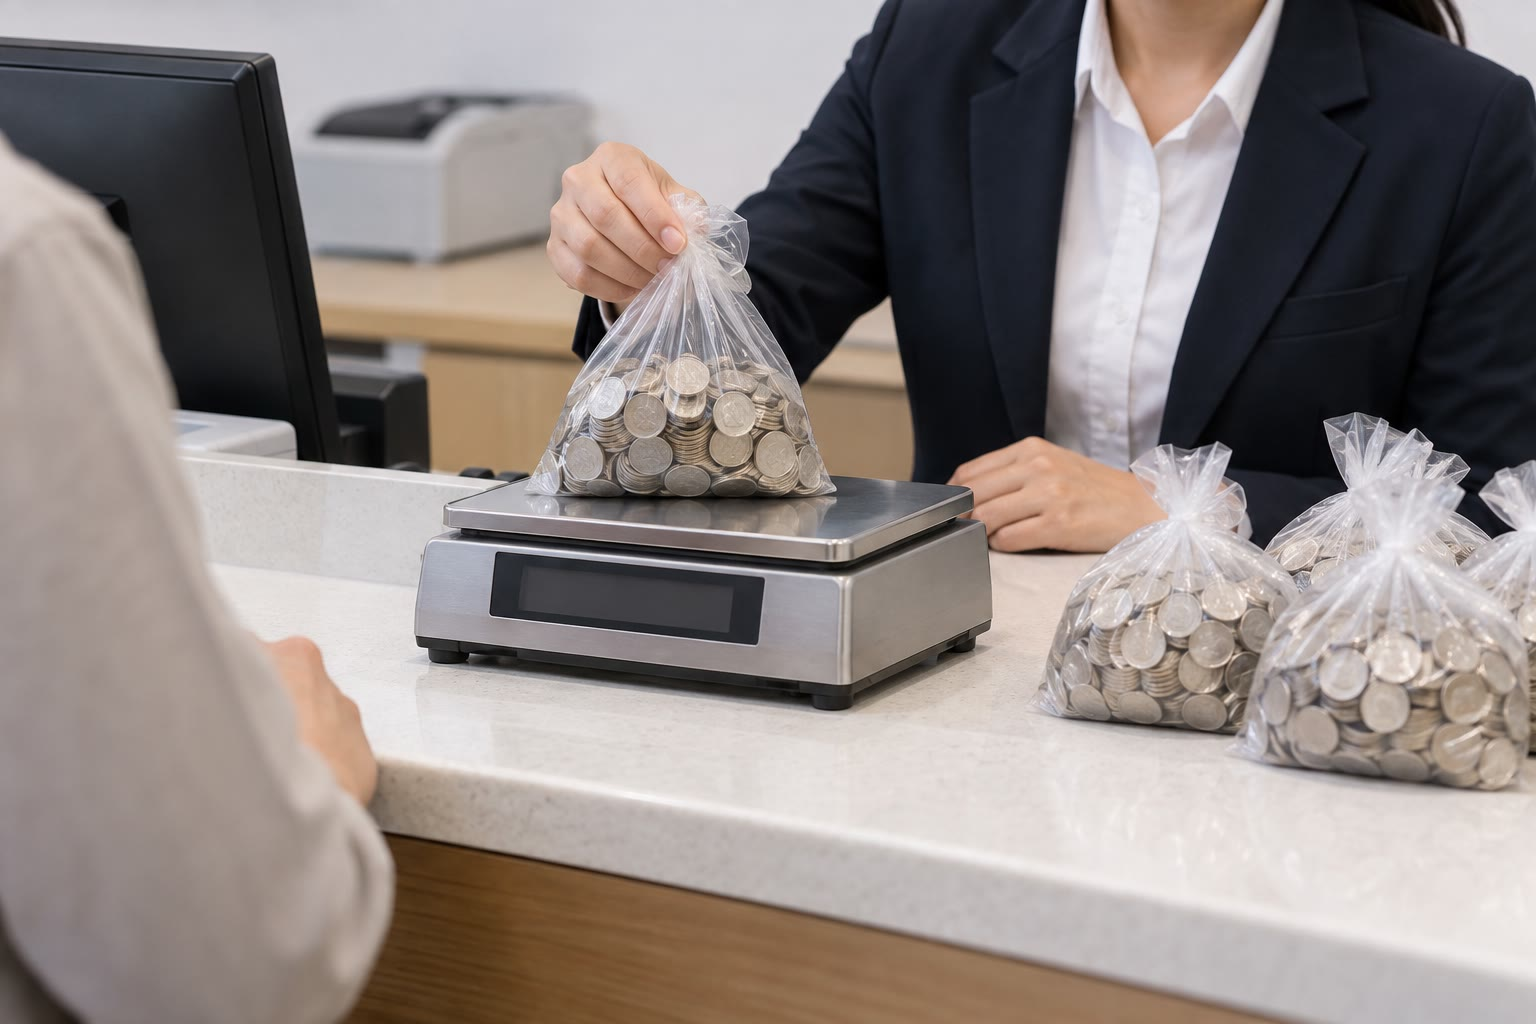
\includegraphics[width=0.55\linewidth]{images/book1/ai/g10-bank-coins.jpg}

{\small बैंक सिक्कों को तौलकर गिनता है। रसायनज्ञ \omterm{def:g7:atoms-and-molecules:atom}{परमाणुओं} को भी
इसी तरह गिनते हैं।}
\end{omfigure}

\section{तौलकर गिनना}

\begin{example}[सिक्कों की थैली]\label{ex:g10:the-mole:coins}
एक सिक्के का द्रव्यमान \qty{7.5}{g} है। इन सिक्कों की एक थैली का द्रव्यमान,
थैली का अपना द्रव्यमान छोड़कर, \qty{1.80}{kg}, यानी \qty{1800}{g}, है।
उसमें इतने सिक्के हैं:
\[
  \frac{\qty{1800}{g}}{\qty{7.5}{g}} = 240 \text{ सिक्के।}
\]
गिनने के लिए बैंक कुल द्रव्यमान को एक सिक्के के द्रव्यमान से भाग देता है।
\end{example}

\begin{example}[पानी की एक चम्मच]\label{ex:g10:the-mole:spoon}
पानी के एक \omterm{def:g7:atoms-and-molecules:molecule}{अणु}, \ce{H2O}, में $2 + 16 = 18$ \omterm{def:g9:inside-the-atom:proton}{न्यूक्लिऑन} होते हैं (प्राकृतिक पानी
लगभग पूरा ऑक्सीजन-16 और हाइड्रोजन-1 \omterm{def:g7:atoms-and-molecules:atom}{परमाणुओं} से बना है), इसलिए उसका द्रव्यमान
लगभग $18 \times \qty{1.67e-27}{kg} = \qty{3.0e-26}{kg}$, यानी
\qty{3.0e-23}{g}, है। इसलिए \qty{5.0}{g} पानी की एक चम्मच में
\[
  \frac{\qty{5.0}{g}}{\qty{3.0e-23}{g}} \approx \num{1.7e23}
  \text{ अणु होते हैं।}
\]
भाग सिक्कों की तरह ही काम करता है, पर उत्तर ऐसी संख्या है जिसकी कोई कल्पना
नहीं कर सकता। रसायनज्ञों को प्रयोगशाला के नमूनों के अनुकूल \omterm{def:g7:atoms-and-molecules:atom}{परमाणुओं} का एक
पैकेट चाहिए।
\end{example}

\begin{definition}[पदार्थ की मात्रा और मोल]\label{def:g10:the-mole:amount}
% ledger: const:NA
किसी नमूने की \emph{पदार्थ की मात्रा}\index{पदार्थ की मात्रा} $n$ उसमें मौजूद
कणों (\omterm{def:g7:atoms-and-molecules:atom}{परमाणु}, \omterm{def:g7:atoms-and-molecules:molecule}{अणु} या \omterm{def:g9:ions:ion}{आयन}, जिन्हें हर बार बताया जाता है) को गिनती है। उसका
मात्रक \emph{मोल}\index{मोल} है, प्रतीक \si{mol}: एक मोल में
ठीक \num{6.02214076e23} कण होते हैं।
\end{definition}

\begin{remark}[एक दर्जन, एक रीम, एक मोल]\label{rem:g10:the-mole:dozen}
\omterm{def:g10:the-mole:amount}{मोल} गिनने का एक मात्रक है, जैसे एक दर्जन अंडे (12) या कागज़ का एक रीम
(500 पन्ने), बस बहुत-बहुत बड़ा। ``पानी के \omterm{def:g7:atoms-and-molecules:molecule}{अणुओं} के दो \omterm{def:g10:the-mole:amount}{मोल}'' का अर्थ है
$2 \times \num{6.02214076e23} = \num{1.20e24}$ \omterm{def:g7:atoms-and-molecules:molecule}{अणु}, ठीक वैसे ही जैसे
``दो दर्जन अंडे'' का अर्थ है 24 अंडे। हमेशा बताइए कि कौन-से कण गिने जा रहे हैं:
ऑक्सीजन \emph{\omterm{def:g7:atoms-and-molecules:molecule}{अणुओं}} \ce{O2} के एक \omterm{def:g10:the-mole:amount}{मोल} में ऑक्सीजन \emph{\omterm{def:g7:atoms-and-molecules:atom}{परमाणुओं}} के
दो \omterm{def:g10:the-mole:amount}{मोल} होते हैं।
\end{remark}

\begin{history}[आवोगाद्रो की परिकल्पना, 1811]
1811 में भौतिकविद आमेदेओ आवोगाद्रो ने प्रस्ताव रखा कि एक ही ताप और दाब पर
अलग-अलग गैसों के समान आयतनों में कणों की संख्या समान होती है। उन्होंने यह भी
समझा कि ऑक्सीजन जैसी गैस दो \omterm{def:g7:atoms-and-molecules:atom}{परमाणुओं} वाले \omterm{def:g7:atoms-and-molecules:molecule}{अणुओं} से बनी है। उनके विचार की
लगभग पचास साल तक उपेक्षा हुई, जब तक कि 1860 में स्तानिस्लाओ कान्निज़्ज़ारो ने
\omterm{def:g7:atoms-and-molecules:atom}{परमाणु} भारों का एक सुसंगत समुच्चय पाने के लिए उसका उपयोग नहीं किया। \omterm{def:g10:the-mole:amount}{मोल} के कणों को
गिनने वाले स्थिरांक का नाम बाद में आवोगाद्रो के नाम पर रखा गया; वे उसका मान कभी
नहीं जान पाए।
\end{history}

\begin{omfigure}
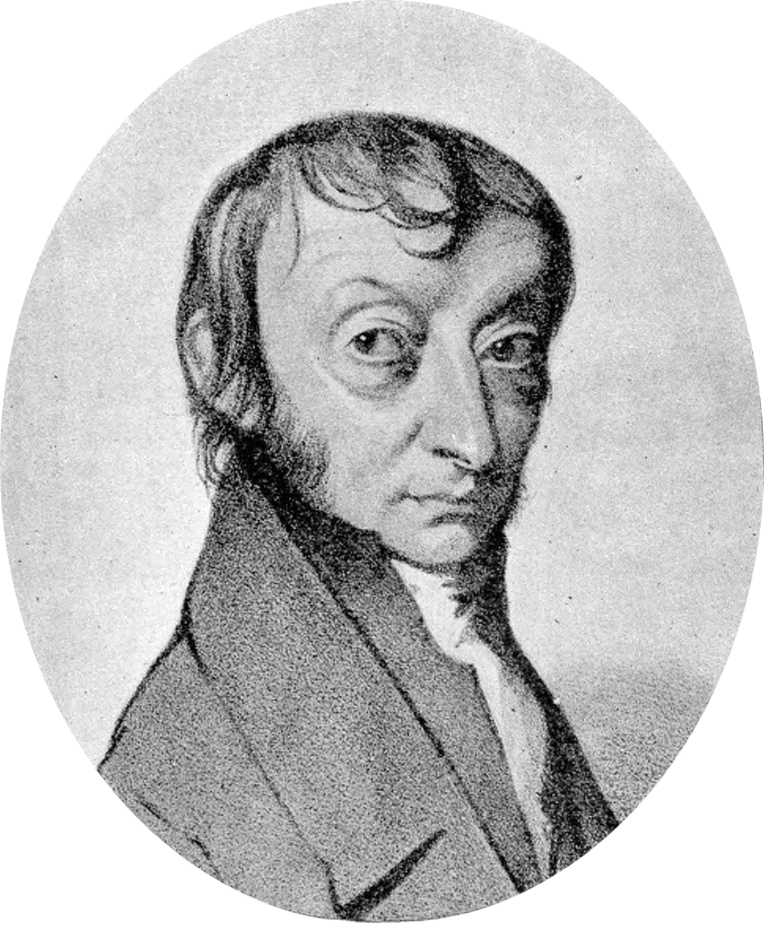
\includegraphics[width=0.26\linewidth]{images/book1/avogadro.jpg}

{\small आमेदेओ आवोगाद्रो (1776--1856)।}
\end{omfigure}

\section{आवोगाद्रो स्थिरांक}

\begin{definition}[आवोगाद्रो स्थिरांक]\label{def:g10:the-mole:avogadro}
% ledger: const:NA
\emph{आवोगाद्रो स्थिरांक}\index{आवोगाद्रो स्थिरांक} $N_A$ प्रति \omterm{def:g10:the-mole:amount}{मोल}
कणों की संख्या है:
\[
  N_A = \qty{6.02214076e23}{mol^{-1}} .
\]
इसका मान सटीक है, परिभाषा द्वारा तय। गणनाओं में इसे पूर्णांकित करके
\qty{6.02e23}{mol^{-1}} लिया जाता है।
\end{definition}

\begin{proposition}[कणों की संख्या और मात्रा]\label{prop:g10:the-mole:number}
$N$ कणों वाले नमूने में \omterm{def:g10:the-mole:amount}{पदार्थ की मात्रा} है
\[
  n = \frac{N}{N_A}, \qquad\text{यानी}\qquad N = n \times N_A .
\]
\end{proposition}

\begin{proof}
हर \omterm{def:g10:the-mole:amount}{मोल} में $N_A$ कण होते हैं, इसलिए $n$ \omterm{def:g10:the-mole:amount}{मोल} में $n \times N_A$ कण होते हैं;
$N_A$ से भाग देने पर $n$ मिलता है।
\end{proof}

\begin{example}[अणु और मोल]\label{ex:g10:the-mole:convert}
एक नमूने में कार्बन डाइऑक्साइड के \num{1.5e24} \omterm{def:g7:atoms-and-molecules:molecule}{अणु} हैं। उसमें कार्बन
डाइऑक्साइड की मात्रा है
$n = \num{1.5e24} / \qty{6.02e23}{mol^{-1}} = \qty{2.5}{mol}$।
उलटे, \qty{0.20}{mol} लोहे में
$N = \qty{0.20}{mol} \times \qty{6.02e23}{mol^{-1}} = \num{1.2e23}$
लोहे के \omterm{def:g7:atoms-and-molecules:atom}{परमाणु} होते हैं।
\end{example}

\begin{remark}[यह संख्या कहाँ से आती है]\label{rem:g10:the-mole:origin}
पचास से अधिक वर्षों तक \omterm{def:g10:the-mole:amount}{मोल} को ठीक \qty{12}{g} कार्बन-12 में \omterm{def:g7:atoms-and-molecules:atom}{परमाणुओं} की
संख्या के रूप में परिभाषित किया जाता था, और $N_A$ को मापना पड़ता था।
2019 से यह संख्या स्वयं तय कर दी गई है, जिससे \omterm{def:g10:the-mole:amount}{मोल} एक शुद्ध गिनती बन गया है।
पुरानी और नई परिभाषाएँ दस करोड़ में एक भाग से भी बेहतर मेल खाती हैं, इसलिए
बारह ग्राम कार्बन-12 में अब भी \omterm{def:g7:atoms-and-molecules:atom}{परमाणुओं} का एक \omterm{def:g10:the-mole:amount}{मोल} होता है, जैसा अगला खंड
जाँचता है।
\end{remark}

\section{मोलर द्रव्यमान}

\begin{definition}[मोलर द्रव्यमान]\label{def:g10:the-mole:molar-mass}
किसी \omterm{def:g6:pure-substances-and-mixtures:species}{रासायनिक स्पीशीज़} का \emph{मोलर द्रव्यमान}\index{मोलर द्रव्यमान} $M$ उसके
कणों के एक \omterm{def:g10:the-mole:amount}{मोल} का द्रव्यमान है, ग्राम प्रति \omterm{def:g10:the-mole:amount}{मोल} (\si{g/mol}) में। किसी
तत्व का मोलर द्रव्यमान, उसके \omterm{def:g9:inside-the-atom:isotope}{समस्थानिकों} के प्राकृतिक \omterm{def:g6:pure-substances-and-mixtures:mixture}{मिश्रण} पर लिया गया, उसका
\emph{परमाणवीय मोलर द्रव्यमान}\index{परमाणवीय मोलर द्रव्यमान} है; वह
\omterm{def:g9:periodic-table-first-look:periodic-table}{आवर्त सारणी} में छपा होता है।
\end{definition}

\begin{example}[कार्बन परमाणुओं का एक मोल]\label{ex:g10:the-mole:carbon}
% ledger: const:NA, const:u
कार्बन-12 के एक \omterm{def:g7:atoms-and-molecules:atom}{परमाणु} का द्रव्यमान लगभग
$12 \times \qty{1.67e-27}{kg} = \qty{2.00e-26}{kg}$ है। उनके एक \omterm{def:g10:the-mole:amount}{मोल} का
द्रव्यमान है
\[
  \qty{2.00e-26}{kg} \times \num{6.02e23} = \qty{1.20e-2}{kg}
  = \qty{12.0}{g}.
\]
\omterm{def:g10:the-mole:amount}{मोल} को इस तरह चुना गया है कि किसी \omterm{def:g7:atoms-and-molecules:atom}{परमाणु} का \omterm{def:g10:the-mole:molar-mass}{मोलर द्रव्यमान}, ग्राम प्रति \omterm{def:g10:the-mole:amount}{मोल} में,
उसकी \omterm{def:g9:inside-the-atom:atomic-number}{द्रव्यमान संख्या} के क़रीब हो: हाइड्रोजन के लिए लगभग \qty{1}{g/mol},
कार्बन के लिए \qty{12}{g/mol}, ऑक्सीजन के लिए \qty{16}{g/mol}।
\end{example}

\begin{omfigure}
% ledger: aw:H, aw:C, aw:N, aw:O, aw:Na, aw:Mg, aw:Al, aw:Si, aw:S, aw:Cl, aw:K, aw:Ca, aw:Fe, aw:Cu, aw:Zn, aw:Au (rounded to 0.1)
\begin{tabular}{lcr@{\qquad}lcr}
\hline
तत्व & प्रतीक & $M$ (\si{g/mol}) & तत्व & प्रतीक & $M$ (\si{g/mol}) \\
\hline
हाइड्रोजन  & \ce{H}  & 1.0  & सिलिकॉन   & \ce{Si} & 28.1 \\
कार्बन    & \ce{C}  & 12.0 & सल्फ़र    & \ce{S}  & 32.1 \\
नाइट्रोजन  & \ce{N}  & 14.0 & क्लोरीन  & \ce{Cl} & 35.5 \\
ऑक्सीजन    & \ce{O}  & 16.0 & पोटैशियम & \ce{K}  & 39.1 \\
सोडियम    & \ce{Na} & 23.0 & कैल्सियम   & \ce{Ca} & 40.1 \\
मैग्नीशियम & \ce{Mg} & 24.3 & लोहा      & \ce{Fe} & 55.8 \\
ऐलुमिनियम & \ce{Al} & 27.0 & ताँबा    & \ce{Cu} & 63.5 \\
          &         &      & सोना      & \ce{Au} & 197.0 \\
\hline
\end{tabular}\par\medskip

{\small आम तत्वों के \omterm{def:g10:the-mole:molar-mass}{परमाणवीय मोलर द्रव्यमान}, \qty{0.1}{g/mol} तक
पूर्णांकित। इस पुस्तक में यही मान उपयोग किए गए हैं।}
\end{omfigure}

\begin{remark}[क्लोरीन 35.5 क्यों है]\label{rem:g10:the-mole:chlorine}
% ledger: iso:Cl35, iso:Cl37
प्राकृतिक क्लोरीन दो \omterm{def:g9:inside-the-atom:isotope}{समस्थानिकों} का \omterm{def:g6:pure-substances-and-mixtures:mixture}{मिश्रण} है: उसके लगभग तीन-चौथाई \omterm{def:g7:atoms-and-molecules:atom}{परमाणु}
क्लोरीन-35 हैं, एक-चौथाई क्लोरीन-37
(\cref{ch:g9:inside-the-atom})। उसका \omterm{def:g10:the-mole:molar-mass}{परमाणवीय मोलर द्रव्यमान} इन हिस्सों से भारित
औसत है, जो 35 और 37 के बीच है: \qty{35.5}{g/mol}।
इसीलिए कुछ \omterm{def:g10:the-mole:molar-mass}{परमाणवीय मोलर द्रव्यमान} पूर्ण संख्याओं से काफ़ी दूर होते हैं।
\end{remark}

\begin{proposition}[अणु का मोलर द्रव्यमान]\label{prop:g10:the-mole:sum}
किसी \omterm{def:g7:atoms-and-molecules:molecule}{अणु} का \omterm{def:g10:the-mole:molar-mass}{मोलर द्रव्यमान} उसके सभी \omterm{def:g7:atoms-and-molecules:atom}{परमाणुओं} के \omterm{def:g10:the-mole:molar-mass}{परमाणवीय मोलर द्रव्यमानों} का योग
है, हर \omterm{def:g7:atoms-and-molecules:atom}{परमाणु} को उतनी बार गिनकर जितनी बार वह सूत्र में आता है। यही
नियम किसी आयनिक ठोस का \omterm{def:g10:the-mole:molar-mass}{मोलर द्रव्यमान} उसकी सूत्र-इकाई से देता है।
\end{proposition}

\begin{proof}
\omterm{def:g7:atoms-and-molecules:molecule}{अणुओं} \ce{A_xB_y} के एक \omterm{def:g10:the-mole:amount}{मोल} में \omterm{def:g7:atoms-and-molecules:atom}{परमाणुओं} \ce{A} के $x$ \omterm{def:g10:the-mole:amount}{मोल} और
\omterm{def:g7:atoms-and-molecules:atom}{परमाणुओं} \ce{B} के $y$ \omterm{def:g10:the-mole:amount}{मोल} होते हैं, और कुछ नहीं; उसका द्रव्यमान उनके द्रव्यमानों का
योग है, $x\,M(\ce{A}) + y\,M(\ce{B})$।
\end{proof}

\begin{example}[तीन मोलर द्रव्यमान]\label{ex:g10:the-mole:three}
% ledger: aw:H, aw:C, aw:O, aw:Na, aw:Cl
\begin{align*}
  M(\ce{H2O}) &= 2 \times 1.0 + 16.0 = \qty{18.0}{g/mol},\\
  M(\ce{NaCl}) &= 23.0 + 35.5 = \qty{58.5}{g/mol},\\
  M(\ce{C12H22O11}) &= 12 \times 12.0 + 22 \times 1.0 + 11 \times 16.0
     = \qty{342.0}{g/mol}.
\end{align*}
आख़िरी सुक्रोस है, यानी मेज़ पर रखी चीनी।
\end{example}

\section{द्रव्यमान से मात्रा और वापस}

\begin{proposition}[द्रव्यमान और मात्रा]\label{prop:g10:the-mole:mass}
द्रव्यमान $m$ वाले नमूने में, जिसकी स्पीशीज़ का \omterm{def:g10:the-mole:molar-mass}{मोलर द्रव्यमान} $M$ है, \omterm{def:g10:the-mole:amount}{पदार्थ की मात्रा} है
\[
  n = \frac{m}{M}, \qquad\text{यानी}\qquad m = n \times M .
\]
$m$ ग्राम में और $M$ ग्राम प्रति \omterm{def:g10:the-mole:amount}{मोल} में हो, तो $n$ \omterm{def:g10:the-mole:amount}{मोल} में आता है।
\end{proposition}

\begin{proof}
हर \omterm{def:g10:the-mole:amount}{मोल} का द्रव्यमान $M$ है, इसलिए $n$ \omterm{def:g10:the-mole:amount}{मोल} का द्रव्यमान $n \times M$ है; यह
बैंक की सिक्का-गिनती ही है, जिसमें \omterm{def:g10:the-mole:amount}{मोल} सिक्का है।
\end{proof}

\begin{method}[द्रव्यमान से कणों की संख्या तक]\label{met:g10:the-mole:mass-to-number}
\begin{enumerate}
  \item स्पीशीज़ का सूत्र लिखिए और सारणी से उसका \omterm{def:g10:the-mole:molar-mass}{मोलर द्रव्यमान} $M$
        निकालिए।
  \item ज़रूरत हो तो द्रव्यमान को ग्राम में बदलिए, फिर $n = m / M$।
  \item अगर कणों की संख्या चाहिए, तो $N = n \times N_A$।
  \item परिमाण की कोटि जाँचिए: किसी छोटे \omterm{def:g7:atoms-and-molecules:molecule}{अणु} के कुछ ग्राम एक \omterm{def:g10:the-mole:amount}{मोल} के
        दसवें भाग की कोटि के होते हैं, लगभग $10^{22}$ से $10^{23}$
        कण।
\end{enumerate}
\end{method}

\begin{omfigure}
\begin{tikzpicture}[font=\small, box/.style={draw=omDef, very thick,
    fill=omDef!8, rounded corners=3pt, minimum width=2.9cm,
    minimum height=1.1cm, align=center}]
  \node[box] (m) at (0,0) {द्रव्यमान $m$\\[1pt] (\si{g})};
  \node[box] (n) at (5,0) {मात्रा $n$\\[1pt] (\si{mol})};
  \node[box] (N) at (10,0) {कणों की\\[1pt] संख्या $N$};
  \draw[-{Stealth[length=7pt]}, thick, omProp] ([yshift=4pt]m.east)
    -- node[above] {$\div M$} ([yshift=4pt]n.west);
  \draw[-{Stealth[length=7pt]}, thick, omProp] ([yshift=-4pt]n.west)
    -- node[below] {$\times M$} ([yshift=-4pt]m.east);
  \draw[-{Stealth[length=7pt]}, thick, omProp] ([yshift=4pt]n.east)
    -- node[above] {$\times N_A$} ([yshift=4pt]N.west);
  \draw[-{Stealth[length=7pt]}, thick, omProp] ([yshift=-4pt]N.west)
    -- node[below] {$\div N_A$} ([yshift=-4pt]n.east);
\end{tikzpicture}

{\small मात्रा $n$ बीच में है: तुला $m$ देती है, \omterm{def:g10:the-mole:molar-mass}{मोलर द्रव्यमान}
$n$ तक ले जाता है, और \omterm{def:g10:the-mole:avogadro}{आवोगाद्रो स्थिरांक} आगे कणों की
संख्या तक।}
\end{omfigure}


\begin{example}[नौ ग्राम पानी]\label{ex:g10:the-mole:nine}
% ledger: aw:H, aw:O, const:NA
\qty{9.0}{g} पानी में कितने \omterm{def:g7:atoms-and-molecules:molecule}{अणु} हैं? $M(\ce{H2O}) =
\qty{18.0}{g/mol}$, इसलिए
\[
  n = \frac{\qty{9.0}{g}}{\qty{18.0}{g/mol}} = \qty{0.50}{mol},
  \qquad
  N = \qty{0.50}{mol} \times \qty{6.02e23}{mol^{-1}}
    = \num{3.0e23} \text{ अणु।}
\]
\end{example}

\begin{example}[बेंच पर एक मोल]\label{ex:g10:the-mole:bench}
% ledger: rho:water, rho:NaCl, rho:sucrose, rho:Fe, aw:H, aw:O, aw:Na, aw:Cl, aw:C, aw:Fe
पानी का एक \omterm{def:g10:the-mole:amount}{मोल} \qty{18.0}{g} है, लगभग एक बड़ा चम्मच। नमक का एक \omterm{def:g10:the-mole:amount}{मोल},
\qty{58.5}{g}, एक छोटी ढेरी है; चीनी का एक \omterm{def:g10:the-mole:amount}{मोल}, \qty{342.0}{g}, एक मग भर देता
है; लोहे का एक \omterm{def:g10:the-mole:amount}{मोल}, \qty{55.8}{g}, \qty{2}{cm} से थोड़ा कम भुजा वाला एक
घन है। चारों में कणों की संख्या एक ही है: चीनी के \omterm{def:g7:atoms-and-molecules:molecule}{अणु} बस पानी के \omterm{def:g7:atoms-and-molecules:molecule}{अणुओं} से कहीं
भारी हैं, और लोहे के \omterm{def:g7:atoms-and-molecules:atom}{परमाणु} कहीं अधिक सघनता से
सजे हैं।
\end{example}

\begin{omfigure}
\begin{tikzpicture}[font=\small, x=0.62cm, y=0.62cm]
  % cubes of true volume, drawn to one common scale: side = cube root of V
  % water 18.09 cm3 -> 2.625 cm; NaCl 26.96 cm3 -> 2.999 cm;
  % sucrose 216.4 cm3 -> 6.004 cm; Fe 7.09 cm3 -> 1.921 cm
  \newcommand{\cube}[4]{% x, side, fill, label
    \pgfmathsetmacro\d{0.35*#2}
    \fill[#3!35, draw=#3!80!black] (#1,0) rectangle ++(#2,#2);
    \fill[#3!20, draw=#3!80!black] (#1,#2) -- ++(\d,\d) -- ++(#2,0)
      -- ++(-\d,-\d) -- cycle;
    \fill[#3!50, draw=#3!80!black] (#1+#2,0) -- ++(\d,\d) -- ++(0,#2)
      -- ++(-\d,-\d) -- cycle;
    \node[below, align=center] at (#1+#2/2,-0.1) {#4};}
  \cube{0}{2.625}{cyan}{पानी\\ \qty{18.0}{g}\\ \qty{18}{cm^3}}
  \cube{4.3}{2.999}{gray}{नमक\\ \qty{58.5}{g}\\ \qty{27}{cm^3}}
  \cube{9}{6.004}{orange}{चीनी\\ \qty{342.0}{g}\\ \qty{216}{cm^3}}
  \cube{18}{1.921}{brown}{लोहा\\ \qty{55.8}{g}\\ \qty{7}{cm^3}}
\end{tikzpicture}

{\small पानी, नमक (सोडियम क्लोराइड), चीनी (सुक्रोस) और लोहे का एक-एक \omterm{def:g10:the-mole:amount}{मोल},
उनके वास्तविक आयतनों के घनों के रूप में, सब एक ही पैमाने पर।
हर एक में \num{6.02e23} कण हैं।}
\end{omfigure}

\section{गैसें: मोलर आयतन}

\begin{definition}[मोलर आयतन]\label{def:g10:the-mole:molar-volume}
किसी गैस का \emph{मोलर आयतन}\index{मोलर आयतन} $V_m$ उस गैस के एक \omterm{def:g10:the-mole:amount}{मोल} द्वारा,
किसी दिए गए ताप और दाब पर, घेरा गया आयतन है।
इसे लीटर प्रति \omterm{def:g10:the-mole:amount}{मोल} (\si{L/mol}) में व्यक्त किया जाता है।
\end{definition}

\begin{proposition}[सभी गैसों का मोलर आयतन एक ही होता है]\label{prop:g10:the-mole:avogadro-law}
% ledger: const:R, const:atm, const:Vm1 (24.1 = R x 293.15 K / 101325 Pa, computed)
किसी दिए गए ताप और दाब पर किसी भी गैस का एक \omterm{def:g10:the-mole:amount}{मोल} लगभग ठीक एक ही आयतन घेरता है,
गैस चाहे कोई भी हो। \qty{20}{\celsius} और
सामान्य वायुमंडलीय दाब पर,
\[
  V_m = \qty{24.1}{L/mol};
\]
\qty{0}{\celsius} और उसी दाब पर $V_m = \qty{22.4}{L/mol}$। तब
आयतन $V$ वाली गैस की मात्रा $n = V / V_m$ होती है।
\end{proposition}

\begin{proof}
यहाँ स्वीकृत: यह 1811 की आवोगाद्रो की परिकल्पना है, जो अब भौतिकी का एक नियम है,
और $V_m$ का मान भौतिकी की पुस्तक में पढ़े जाने वाले गैस नियमों से
निकलता है।
\end{proof}

\begin{omfigure}
\begin{tikzpicture}[font=\small]
  \foreach \x/\g/\m/\c in {0/{\ce{H2}}/2.0/cyan, 4/{\ce{O2}}/32.0/red,
                           8/{\ce{CO2}}/44.0/gray} {
    \draw[thick, black!60] (\x,-0.25) -- (\x,-1.1);
    \shade[ball color=\c!45, draw=\c!70!black] (\x,0.55) ellipse (1.05 and 1.2);
    \fill[\c!70!black] (\x-0.12,-0.68) -- (\x+0.12,-0.68) -- (\x,-0.55) -- cycle;
    \node[align=center] at (\x,-1.65) {\g\ का 1 mol\\ \qty{\m}{g},
      \qty{24.1}{L}};
  }
\end{tikzpicture}

{\small \qty{20}{\celsius} पर तीन गुब्बारे, हर एक में किसी अलग गैस का एक \omterm{def:g10:the-mole:amount}{मोल}।
आयतन एक ही हैं; द्रव्यमान नहीं।}
\end{omfigure}


\begin{example}[कार्बन डाइऑक्साइड का गुब्बारा]\label{ex:g10:the-mole:balloon}
% ledger: aw:C, aw:O
एक गुब्बारे में \qty{20}{\celsius} पर \qty{2.4}{L} कार्बन डाइऑक्साइड है।
उसकी मात्रा $n = \qty{2.4}{L} / \qty{24.1}{L/mol} = \qty{0.10}{mol}$ है,
और उसका द्रव्यमान $m = \qty{0.10}{mol} \times \qty{44.0}{g/mol} =
\qty{4.4}{g}$। हाइड्रोजन से भरे उसी गुब्बारे में भी उतनी ही
\qty{0.10}{mol} गैस होगी, पर केवल \qty{0.20}{g}।
\end{example}

\begin{remark}[भारी और हल्की गैसें]\label{rem:g10:the-mole:heavy}
चूँकि किसी भी गैस के एक लीटर में \omterm{def:g10:the-mole:amount}{पदार्थ की मात्रा} एक ही होती है, गैस के एक लीटर
का द्रव्यमान उसके \omterm{def:g10:the-mole:molar-mass}{मोलर द्रव्यमान} के समानुपाती होता है। \omterm{def:g4:air-a-mixture-of-gases:air}{वायु}, जो लगभग चार-पाँचवाँ
भाग नाइट्रोजन (\qty{28.0}{g/mol}) और पाँचवाँ भाग ऑक्सीजन
(\qty{32.0}{g/mol}) का \omterm{def:g6:pure-substances-and-mixtures:mixture}{मिश्रण} है, लगभग
\qty{29}{g/mol} \omterm{def:g10:the-mole:molar-mass}{मोलर द्रव्यमान} वाली गैस जैसा व्यवहार करती है। अधिक \omterm{def:g10:the-mole:molar-mass}{मोलर द्रव्यमान}
वाली गैस, जैसे कार्बन डाइऑक्साइड
(\qty{44.0}{g/mol}), \omterm{def:g4:air-a-mixture-of-gases:air}{वायु} से घनी होती है और बंद तहख़ाने की तली में जमा होती
है; कम \omterm{def:g10:the-mole:molar-mass}{मोलर द्रव्यमान} वाली गैस, जैसे हीलियम
(\qty{4.0}{g/mol}), ऊपर उठती है।
\end{remark}

\section{अभ्यास}

\begin{exercise}[$\star$]\label{exo:g10:the-mole:1}
डाइऑक्सीजन \ce{O2}, डाइनाइट्रोजन \ce{N2}, मेथेन \ce{CH4}, अमोनिया \ce{NH3} और
कार्बन डाइऑक्साइड \ce{CO2} के \omterm{def:g10:the-mole:molar-mass}{मोलर द्रव्यमान} निकालिए।
\end{exercise}

\begin{exercise}[$\star$]\label{exo:g10:the-mole:2}
\qty{36.0}{g} पानी में पदार्थ की कितनी मात्रा है? \qty{4.0}{g} मेथेन
में?
\end{exercise}

\begin{exercise}[$\star$]\label{exo:g10:the-mole:3}
सोडियम क्लोराइड \ce{NaCl} के \qty{0.25}{mol} का द्रव्यमान कितना है?
कार्बन डाइऑक्साइड के \qty{2.0}{mol} का?
\end{exercise}

\begin{exercise}[$\star$]\label{exo:g10:the-mole:4}
डाइऑक्सीजन के \qty{0.50}{mol} में कितने \omterm{def:g7:atoms-and-molecules:molecule}{अणु} हैं? लोहे की कितनी मात्रा में
लोहे के \num{3.0e24} \omterm{def:g7:atoms-and-molecules:atom}{परमाणु} होते हैं?
\end{exercise}

\begin{exercise}[$\star$]\label{exo:g10:the-mole:5}
\qty{20}{\celsius} और सामान्य वायुमंडलीय दाब पर डाइनाइट्रोजन का \qty{0.50}{mol}
कितना आयतन घेरता है? उस गैस के \qty{12}{L} में डाइऑक्सीजन की कितनी मात्रा
है?
\end{exercise}

\begin{exercise}[$\star\star$]\label{exo:g10:the-mole:6}
पानी की एक बूँद का आयतन \qty{0.050}{mL} है, और \qty{1}{mL} पानी का
द्रव्यमान \qty{1.0}{g} है। बूँद में पानी के कितने \omterm{def:g7:atoms-and-molecules:molecule}{अणु}
हैं?
\end{exercise}

\begin{exercise}[$\star\star$]\label{exo:g10:the-mole:7}
किसमें अधिक \omterm{def:g7:atoms-and-molecules:atom}{परमाणु} हैं, \qty{10}{g} ऐलुमिनियम में या \qty{10}{g}
लोहे में? पहले बिना गणना के समझाइए, फिर गणना करके जाँचिए।
\end{exercise}

\begin{exercise}[$\star\star$]\label{exo:g10:the-mole:8}
\qty{20}{\celsius} पर कार्बन डाइऑक्साइड के एक लीटर का और डाइनाइट्रोजन के एक लीटर
का द्रव्यमान निकालिए। जिस बंद तहख़ाने में अंगूर का रस किण्वित हो रहा हो, उसकी तली
में कार्बन डाइऑक्साइड क्यों जमा होती है?
\end{exercise}

\begin{exercise}[$\star\star$]\label{exo:g10:the-mole:9}
$m$, $n$, $N$ वाले तीन खानों के चित्र की मदद से ग्लूकोस \ce{C6H12O6} के
\num{1.0e22} \omterm{def:g7:atoms-and-molecules:molecule}{अणुओं} का द्रव्यमान बताइए। जिन दो
तीरों का पालन किया, उन्हें लिखिए।
\end{exercise}

\begin{exercise}[$\star\star$]\label{exo:g10:the-mole:10}
चीनी (सुक्रोस, \ce{C12H22O11}) की एक डली का द्रव्यमान \qty{5.0}{g} है।
उसमें सुक्रोस की मात्रा निकालिए, फिर सुक्रोस के \omterm{def:g7:atoms-and-molecules:molecule}{अणुओं} की संख्या, फिर
कार्बन \omterm{def:g7:atoms-and-molecules:atom}{परमाणुओं} की संख्या।
\end{exercise}

\begin{exercise}[$\star\star$]\label{exo:g10:the-mole:11}
किसमें \omterm{def:g7:atoms-and-molecules:molecule}{अणुओं} की मात्रा अधिक है: \qty{1.0}{kg} पानी
\ce{H2O} में या \qty{1.0}{kg} एथेनॉल \ce{C2H6O} में? कितने गुना?
\end{exercise}

\begin{exercise}[$\star\star\star$]\label{exo:g10:the-mole:12}
सोने की एक अँगूठी का द्रव्यमान \qty{5.0}{g} है; उसके द्रव्यमान का तीन-चौथाई भाग
सोना है, बाकी ताँबा। उसमें सोने के कितने \omterm{def:g7:atoms-and-molecules:atom}{परमाणु} हैं? ताँबे के कितने
\omterm{def:g7:atoms-and-molecules:atom}{परमाणु}? अँगूठी में किस \omterm{def:g9:periodic-table-first-look:metal}{धातु} के \omterm{def:g7:atoms-and-molecules:atom}{परमाणु} अधिक हैं?
\end{exercise}

\begin{exercise}[$\star\star\star$]\label{exo:g10:the-mole:13}
एक कक्षा का माप \qty{8.0}{m} गुणा \qty{6.0}{m} गुणा \qty{3.0}{m} है, और
उसकी \omterm{def:g4:air-a-mixture-of-gases:air}{वायु} \qty{20}{\celsius} पर है।
\begin{enumerate}
  \item उसमें गैस की कितनी मात्रा है ($\qty{1}{m^3} =
        \qty{1000}{L}$)? कितने \omterm{def:g7:atoms-and-molecules:molecule}{अणु}?
  \item हर सौ में 78 \omterm{def:g7:atoms-and-molecules:molecule}{अणु} डाइनाइट्रोजन, 21 डाइऑक्सीजन और 1
        आर्गन (\qty{40.0}{g/mol}) मानकर \omterm{def:g4:air-a-mixture-of-gases:air}{वायु} का माध्य
        \omterm{def:g10:the-mole:molar-mass}{मोलर द्रव्यमान} निकालिए।
  \item कमरे की \omterm{def:g4:air-a-mixture-of-gases:air}{वायु} का द्रव्यमान कितना है?
\end{enumerate}
\end{exercise}

\begin{exercise}[$\star\star\star$]\label{exo:g10:the-mole:14}
शुद्ध सिलिकॉन के एक गोले का द्रव्यमान ठीक \qty{1.000}{kg} है।
\begin{enumerate}
  \item उसमें सिलिकॉन के कितने \omterm{def:g7:atoms-and-molecules:atom}{परमाणु} हैं?
  \item सिलिकॉन के एक \omterm{def:g7:atoms-and-molecules:atom}{परमाणु} का द्रव्यमान निकालिए।
  \item 2019 से पहले \omterm{def:g10:the-mole:avogadro}{आवोगाद्रो स्थिरांक} तय नहीं था, बल्कि मापा जाता था।
        समझाइए कि ऐसे गोले के \omterm{def:g7:atoms-and-molecules:atom}{परमाणुओं} की एक स्वतंत्र गिनती, जिसकी मात्रा उसके
        द्रव्यमान से ज्ञात है, उसका मान कैसे देगी।
\end{enumerate}
\end{exercise}

\begin{exercise}[$\star\star\star$]\label{exo:g10:the-mole:15}
% ledger: iso:Cl35, iso:Cl37
प्राकृतिक क्लोरीन में \qty{75.8}{\percent} \omterm{def:g7:atoms-and-molecules:atom}{परमाणु} क्लोरीन-35 के हैं, जिसका
\omterm{def:g10:the-mole:molar-mass}{मोलर द्रव्यमान} \qty{35.0}{g/mol} के बहुत क़रीब है, और \qty{24.2}{\percent}
क्लोरीन-37 के, जिसका \omterm{def:g10:the-mole:molar-mass}{मोलर द्रव्यमान} \qty{37.0}{g/mol} के बहुत क़रीब है।
प्राकृतिक क्लोरीन का \omterm{def:g10:the-mole:molar-mass}{परमाणवीय मोलर द्रव्यमान} निकालिए, और उसकी तुलना
सारणी के मान से कीजिए।
\end{exercise}

\section{समस्या: केल्विन का पानी का गिलास}

\begin{problem}[{सप्ताहांत समस्या --- पानी का एक गिलास समुद्र में उँडेलिए, उसके सारे
महासागरों में मिल जाने का इंतज़ार कीजिए, और फिर गिलास भरिए: पहले के कितने
अणु वापस आते हैं?}]
\label{pb:g10:the-mole:1}
% ledger: ocean:volume, rho:water, const:NA, aw:H, aw:O
एक प्रसिद्ध विचार-प्रयोग, जिसे अक्सर भौतिकविद लॉर्ड केल्विन से जोड़ा जाता है,
इस प्रकार है। पानी के एक गिलास के हर \omterm{def:g7:atoms-and-molecules:molecule}{अणु} पर निशान लगाइए, गिलास को समुद्र में
उँडेल दीजिए, और तब तक इंतज़ार कीजिए जब तक निशान वाले \omterm{def:g7:atoms-and-molecules:molecule}{अणु} दुनिया के सारे
महासागरों में समान रूप से न फैल जाएँ। फिर गिलास को समुद्र में कहीं भी फिर से
डुबोइए। क्या उसमें निशान वाले कोई \omterm{def:g7:atoms-and-molecules:molecule}{अणु} वापस आएँगे? गिलास में
\qty{250}{mL} आता है, और \qty{1}{mL} पानी का द्रव्यमान \qty{1.0}{g} है।
महासागरों में लगभग \qty{1.335e9}{km^3} पानी है। गिनती के लिए समुद्र के पानी
को शुद्ध पानी मानिए।

\medskip
\noindent\textbf{भाग I --- गिलास में पानी।}
\begin{enumerate}
  \item पानी का \omterm{def:g10:the-mole:molar-mass}{मोलर द्रव्यमान} निकालिए।
  \item गिलास के पानी का द्रव्यमान कितना है?
  \item गिलास में पानी के \omterm{def:g7:atoms-and-molecules:molecule}{अणुओं} की मात्रा निकालिए।
  \item गिलास में हाइड्रोजन \omterm{def:g7:atoms-and-molecules:atom}{परमाणुओं} की कितनी मात्रा है? ऑक्सीजन
        \omterm{def:g7:atoms-and-molecules:atom}{परमाणुओं} की?
\end{enumerate}

\medskip
\noindent\textbf{भाग II --- गिलास के \omterm{def:g7:atoms-and-molecules:molecule}{अणु}।}
\begin{enumerate}[resume]
  \item गिलास में पानी के कितने \omterm{def:g7:atoms-and-molecules:molecule}{अणु} हैं?
  \item पानी के एक \omterm{def:g7:atoms-and-molecules:molecule}{अणु} का द्रव्यमान ग्राम में निकालिए।
  \item 5 और 6 के उत्तरों को गुणा करके जाँचिए: गुणनफल क्या होना
        चाहिए?
  \item दिन-रात हर सेकंड एक \omterm{def:g7:atoms-and-molecules:molecule}{अणु} गिनें, तो गिलास के \omterm{def:g7:atoms-and-molecules:molecule}{अणुओं} को गिनने में कितने वर्ष
        लगेंगे? (एक वर्ष लगभग \qty{3.16e7}{s} का होता है।)
\end{enumerate}

\medskip
\noindent\textbf{भाग III --- महासागर।}
\begin{enumerate}[resume]
  \item महासागरों के आयतन को घन मीटर में बदलिए
        ($\qty{1}{km^3} = \qty{e9}{m^3}$), फिर लीटर में।
  \item निशान वाले \omterm{def:g7:atoms-and-molecules:molecule}{अणुओं} के समान रूप से फैल जाने पर महासागर के हर लीटर में
        उनमें से कितने होंगे?
  \item दूसरा गिलास निशान वाले कितने \omterm{def:g7:atoms-and-molecules:molecule}{अणु} वापस लाता है?
  \item दूसरी विधि। एक लीटर का द्रव्यमान \qty{1.0}{kg} लेकर महासागरों में पानी
        की मात्रा निकालिए।
  \item महासागर के पानी के सभी \omterm{def:g7:atoms-and-molecules:molecule}{अणुओं} का कितना भिन्न निशान वाला है?
  \item इस भिन्न को दूसरे गिलास के \omterm{def:g7:atoms-and-molecules:molecule}{अणुओं} की संख्या से गुणा कीजिए, और
        प्रश्न 11 के उत्तर से तुलना कीजिए।
\end{enumerate}

\medskip
\noindent\textbf{भाग IV --- इसका अर्थ।}
\begin{enumerate}[resume]
  \item महासागरों के पानी से \qty{250}{mL} के कितने गिलास भरे
        जा सकते हैं?
  \item इस संख्या की तुलना एक गिलास के \omterm{def:g7:atoms-and-molecules:molecule}{अणुओं} की संख्या से कीजिए।
        एक वाक्य में समझाइए कि दूसरा गिलास निशान वाले इतने अधिक \omterm{def:g7:atoms-and-molecules:molecule}{अणु}
        क्यों वापस लाता है।
  \item निशान वाला एक अकेला \omterm{def:g7:atoms-and-molecules:molecule}{अणु} वापस लाने के लिए औसतन समुद्र के पानी का कितना
        आयतन निकालना होगा? \qty{0.05}{mL} की एक बूँद से
        तुलना कीजिए।
  \item प्रश्न 11 के उत्तर में बहुत-से अंक हैं। उसे केवल परिमाण की
        कोटि के रूप में क्यों दिया जाना चाहिए? दो कारण बताइए।
  \item अंतिम उत्तर बताइए: पहले गिलास के लगभग कितने \omterm{def:g7:atoms-and-molecules:molecule}{अणु} दूसरे में
        वापस आते हैं?
\end{enumerate}
\end{problem}
